% === START SEGMENT 1 ===
\documentclass[11pt,a4paper]{article}
\usepackage[margin=1in]{geometry}
\usepackage{mathpazo}
\usepackage{amsmath,amssymb}
\usepackage{booktabs}
\usepackage{graphicx}
\usepackage{hyperref}
\usepackage{tikz}
\usetikzlibrary{shapes.geometric,arrows.meta,positioning,calc,fit,backgrounds}
\usepackage{pgfplots}
\pgfplotsset{compat=1.18}
\usepackage{multirow}
\usepackage{xcolor}
\usepackage{fancyhdr}
\usepackage{enumitem}
\usepackage{tabularx}
\usepackage{float}
\definecolor{robustblue}{HTML}{1A73E8}
\definecolor{robustdark}{HTML}{0D47A1}
\definecolor{robustgrey}{HTML}{F5F5F5}
\definecolor{socgreen}{HTML}{2E7D32}
\definecolor{llmred}{HTML}{C62828}
\definecolor{pqcpurple}{HTML}{6A1B9A}
\hypersetup{colorlinks=true,linkcolor=robustblue,citecolor=robustblue,urlcolor=robustdark}
\pagestyle{fancy}
\fancyhf{}
\fancyhead[L]{\small\textsc{RobustIDPS.ai --- Technical Documentation v2}}
\fancyhead[R]{\small\thepage}
\fancyfoot[C]{\small DOI: 10.5281/zenodo.19129512}
\renewcommand{\headrulewidth}{0.4pt}
\renewcommand{\footrulewidth}{0.2pt}
\title{%
  \vspace{-1cm}
  {\LARGE\bfseries RobustIDPS.ai}\\[6pt]
  {\large An Adversarially Robust AI/ML Security Platform with 13+ Neural\\
   Network Models, SOC Intelligence, and LLM Security Testing}}
\author{%
  \textbf{Roger Nick Anaedevha} --- \href{mailto:roger@robustidps.ai}{roger@robustidps.ai}\\
  ICIS, MEPhI, Moscow, Russia\\[6pt]
  Supervised by \textbf{Alexander Gennadievich Trofimov} --- \href{mailto:agtrofimov@robustidps.ai}{agtrofimov@robustidps.ai}\\
  ICIS, MEPhI\\[8pt]
  \normalsize DOI: \texttt{10.5281/zenodo.19129512}}
\date{April 2026}
\begin{document}
\maketitle
\thispagestyle{fancy}
%% ================================================================
%%  ABSTRACT
%% ================================================================
\begin{abstract}
\noindent
RobustIDPS.ai is a comprehensive, open-source AI-native intrusion detection and prevention platform comprising 46 interconnected pages organised into 9 functional groups, integrating more than 13 machine learning and deep learning models for network traffic classification across 34 attack classes and 83 engineered features.  This documentation details every subsystem of the platform.  The SOC Intelligence Suite (6 pages) provides agentic auto-investigation, natural language threat hunting, automated incident reporting, threat intelligence enrichment, IDS rule generation, and CVE vulnerability mapping.  The LLM Security Testing module (5 pages) evaluates prompt injection, jailbreak techniques, RAG poisoning, multi-agent chain attacks, and data poisoning with a 94.5\% overall detection rate.  MLSecOps compliance is ensured through integrated MITRE ATT\&CK mapping, OWASP LLM Top~10 scoring, and NIST AI RMF dashboards.  Novel contributions include a Multi-Agent Post-Quantum Cryptography IDS (PQC-IDS) with four cooperative agents, a unified Continual Learning--Reinforcement Learning (CL-RL) framework sharing Fisher information between EWC regularisation and adversarial training, and user identity management via RobustID profiles.  The platform is deployed as a Progressive Web Application (PWA) with Docker Compose orchestration, PostgreSQL persistence, and Redis caching.  Three purpose-built validation PCAP datasets provide controlled ground truth for regression testing across all detection models.
\end{abstract}
%% ================================================================
%%  SECTION 1 --- INTRODUCTION
%% ================================================================
\section{Introduction}
\label{sec:introduction}
The rapid integration of artificial intelligence into cybersecurity operations has produced a new generation of commercial platforms: CrowdStrike Charlotte AI provides conversational threat analysis atop the Falcon sensor suite; SentinelOne Purple AI augments endpoint detection with natural language querying; Microsoft Security Copilot embeds GPT-4 reasoning into the Defender ecosystem; and Google Sec-Gemini leverages multimodal foundation models for threat intelligence synthesis.  While these platforms demonstrate the operational value of AI-augmented security, they share three fundamental limitations: (i)~proprietary, single-vendor LLM integration that prevents cross-provider benchmarking; (ii)~absence of systematic adversarial robustness evaluation for the ML components themselves; and (iii)~no support for post-quantum cryptographic traffic analysis.

RobustIDPS.ai addresses these gaps as an open-source, academically rigorous alternative.  The platform integrates more than 13 neural network architectures---from a seven-branch surrogate ensemble with Monte Carlo dropout uncertainty quantification to a Mamba-based state-space detector and a stochastic differential equation temporal graph neural network---within a unified detection pipeline.  Adversarial robustness is evaluated against six attack families (FGSM, PGD, C\&W, DeepFool, Gaussian noise, label-masking poisoning) at configurable perturbation budgets.  Continual learning via Elastic Weight Consolidation with experience replay enables adaptation to concept drift without catastrophic forgetting, while a Constrained Policy Optimisation agent provides autonomous graduated response.

Unique among both commercial and open-source alternatives, RobustIDPS.ai offers integrated LLM attack surface testing (prompt injection, jailbreak, RAG poisoning, multi-agent chain attacks, data poisoning), multi-provider LLM support (Claude, GPT-4o, Gemini, DeepSeek, Llama), and a Multi-Agent PQC-IDS module for post-quantum traffic classification.  The platform is deployed as a 46-page Progressive Web Application with full SOC Intelligence capabilities, MLSecOps compliance dashboards, and three validation PCAP datasets for reproducible benchmarking.
%% ================================================================
%%  SECTION 2 --- SYSTEM ARCHITECTURE
%% ================================================================
\section{System Architecture}
\label{sec:architecture}
RobustIDPS.ai is structured as a React 18 single-page application communicating with a Flask/Python backend through 60+ RESTful API endpoints and persistent WebSocket channels for real-time monitoring.  The platform is orchestrated via Docker Compose with PostgreSQL for relational persistence, Redis for caching and session management, and Celery for asynchronous task execution.  PWA support enables offline-capable deployment with service worker caching.

\subsection{Architectural Overview}
Figure~\ref{fig:architecture} presents the high-level architecture incorporating the SOC Intelligence and LLM Security layers.
\begin{figure}[H]
\centering
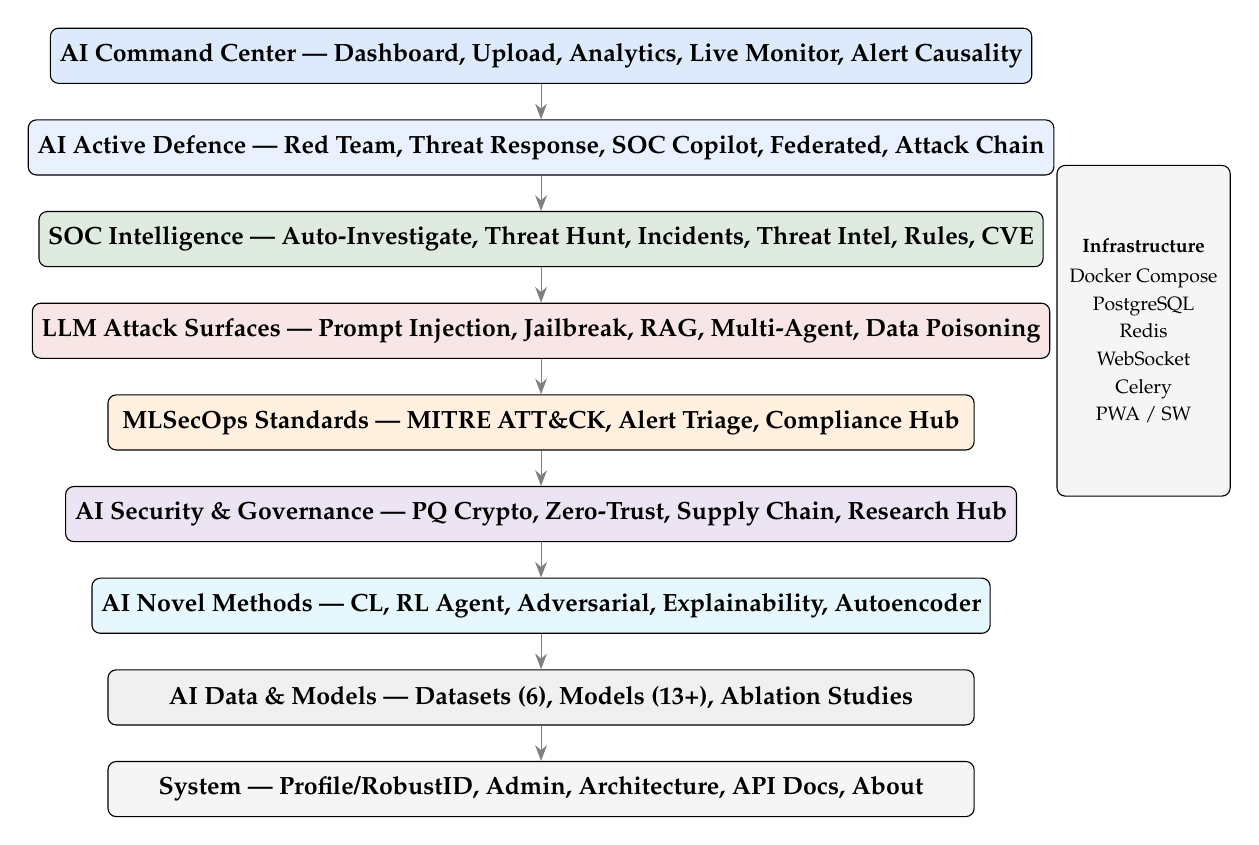
\begin{tikzpicture}[
  node distance=0.45cm and 0.8cm,
  every node/.style={font=\small},
  layer/.style={draw, rounded corners=3pt, minimum width=11cm,
    minimum height=0.7cm, align=center, font=\small\bfseries},
  sublayer/.style={draw, rounded corners=2pt, minimum width=5cm,
    minimum height=0.6cm, align=center, font=\scriptsize}]
\node[layer, fill=robustblue!15] (ui)
  {AI Command Center --- Dashboard, Upload, Analytics, Live Monitor, Alert Causality};
\node[layer, fill=robustblue!10, below=of ui] (defence)
  {AI Active Defence --- Red Team, Threat Response, SOC Copilot, Federated, Attack Chain};
\node[layer, fill=socgreen!15, below=of defence] (soc)
  {SOC Intelligence --- Auto-Investigate, Threat Hunt, Incidents, Threat Intel, Rules, CVE};
\node[layer, fill=llmred!12, below=of soc] (llm)
  {LLM Attack Surfaces --- Prompt Injection, Jailbreak, RAG, Multi-Agent, Data Poisoning};
\node[layer, fill=orange!12, below=of llm] (mlsecops)
  {MLSecOps Standards --- MITRE ATT\&CK, Alert Triage, Compliance Hub};
\node[layer, fill=pqcpurple!12, below=of mlsecops] (security)
  {AI Security \& Governance --- PQ Crypto, Zero-Trust, Supply Chain, Research Hub};
\node[layer, fill=cyan!10, below=of security] (novel)
  {AI Novel Methods --- CL, RL Agent, Adversarial, Explainability, Autoencoder};
\node[layer, fill=gray!12, below=of novel] (data)
  {AI Data \& Models --- Datasets (6), Models (13+), Ablation Studies};
\node[layer, fill=gray!8, below=of data] (system)
  {System --- Profile/RobustID, Admin, Architecture, API Docs, About};
\node[draw, rounded corners=3pt, fill=robustgrey, minimum width=2.2cm,
      minimum height=4.2cm, align=center, font=\scriptsize,
      right=0.6cm of $(soc.east)!0.5!(mlsecops.east)$] (infra) {
  \textbf{Infrastructure}\\[3pt]Docker Compose\\[2pt]PostgreSQL\\[2pt]Redis\\[2pt]WebSocket\\[2pt]Celery\\[2pt]PWA / SW};
\foreach \src/\dst in {ui/defence, defence/soc, soc/llm, llm/mlsecops,
                        mlsecops/security, security/novel, novel/data, data/system} {
  \draw[-{Stealth[length=2mm]}, gray] (\src) -- (\dst);}
\end{tikzpicture}
\caption{High-level system architecture of RobustIDPS.ai showing all 9 functional groups and supporting infrastructure.}
\label{fig:architecture}
\end{figure}

\subsection{Functional Group Summary}
Table~\ref{tab:groups} summarises the nine groups, their page counts, and key features.
\begin{table}[H]
\centering
\caption{RobustIDPS.ai functional groups (46 pages across 9 groups).}
\label{tab:groups}
\small
\begin{tabular}{@{}llcl@{}}
\toprule
\textbf{Group} & \textbf{Pages} & \textbf{Key Features} \\
\midrule
AI Command Center     & 5 & Dashboard, Upload, Analytics, Live Monitor, Alert Causality \\
AI Active Defence     & 5 & Red Team, Threat Response, SOC Copilot, Federated, Attack Chain \\
SOC Intelligence      & 6 & Auto-Investigate, Threat Hunt, Incidents, Threat Intel, Rules, CVE \\
LLM Attack Surfaces   & 5 & Prompt Injection, Jailbreak, RAG, Multi-Agent, Data Poisoning \\
MLSecOps Standards    & 3 & MITRE ATT\&CK, Alert Triage, Compliance Hub \\
AI Security \& Gov    & 4 & PQ Crypto, Zero-Trust, Supply Chain, Research Hub \\
AI Novel Methods      & 5 & Continual Learning, RL Agent, Adversarial, Explainability, Autoencoder \\
AI Data \& Models     & 3 & Datasets, Models (13+), Ablation \\
System                & 5 & Profile, Admin, Architecture, API Docs, About \\
\midrule
\textbf{Total}        & \textbf{46} & \\
\bottomrule
\end{tabular}
\end{table}
The backend exposes 60+ API endpoints covering detection, analysis, LLM integration, user management, and system administration.  WebSocket channels provide sub-second push notifications for live monitoring, alert causality updates, and detection progress.  Docker Compose orchestration enables single-command deployment with environment-based configuration for development, staging, and production profiles.
%% ================================================================
%%  SECTION 3 --- DETECTION MODELS
%% ================================================================
\section{Detection Models}
\label{sec:models}
RobustIDPS.ai integrates more than 13 neural network architectures, each designed to address specific aspects of the intrusion detection problem.  Table~\ref{tab:model_performance} summarises performance across the primary evaluation metrics.

\subsection{Model Descriptions}
\begin{enumerate}[leftmargin=*,label=\textbf{\arabic*.}]
  \item \textbf{SurrogateIDS (7-Branch Ensemble)} --- Seven parallel classifier branches with shared feature extraction, MC dropout ($T{=}20$) uncertainty quantification, and temperature-scaled calibration.
  \item \textbf{CL-RL Unified} --- EWC continual learning with Constrained Policy Optimisation for joint detection and response, sharing Fisher information via $\beta{=}0.7$.
  \item \textbf{CT-TGNN} --- Continuous-time temporal graph neural network modelling host-level communication dynamics with attention-based temporal aggregation.
  \item \textbf{SDE-TGNN} --- Extends CT-TGNN with stochastic differential equations for continuous-time graph evolution under uncertainty.
  \item \textbf{MambaShield} --- Mamba state-space architecture providing linear-time sequence processing for high-throughput flow classification.
  \item \textbf{Stochastic Transformer} --- Transformer encoder with stochastic depth and MC dropout for calibrated uncertainty-aware detection.
  \item \textbf{FedGTD} --- Byzantine-resilient federated model using geometric trimmed deviation aggregation, tolerating up to 30\% malicious participants.
  \item \textbf{CyberSecLLM} --- Fine-tuned LLM for traffic classification with chain-of-thought reasoning, supporting Claude, GPT-4o, Gemini, DeepSeek, and Llama backends.
  \item \textbf{Multi-Agent PQC-IDS} --- Four cooperative agents (Traffic Analyst, PQC Specialist, Anomaly Detector, Coordinator) with attention-weighted fusion for post-quantum traffic analysis.
  \item \textbf{Neural ODE} --- Continuous-depth residual network using neural ordinary differential equations for adaptive computation based on input complexity.
  \item \textbf{Optimal Transport} --- Wasserstein-distance-based classifier leveraging optimal transport theory for distribution-aware anomaly detection.
  \item \textbf{Variational Autoencoder} --- Deep generative model for unsupervised anomaly detection via reconstruction error in latent space.
  \item \textbf{Adversarial Autoencoder} --- Adversarial training with autoencoder reconstruction for robust feature learning under input perturbation.
\end{enumerate}

\subsection{Performance Summary}
\begin{table}[H]
\centering
\caption{Detection model performance on the combined validation set (clean conditions). Accuracy and F1 are macro-averaged; ECE is expected calibration error; latency is per-flow on a single CPU core.}
\label{tab:model_performance}
\small
\begin{tabular}{@{}lcccc@{}}
\toprule
\textbf{Model} & \textbf{Accuracy} & \textbf{F1} & \textbf{ECE} & \textbf{Latency} \\
\midrule
SurrogateIDS (7-Branch)   & 97.8\% & 0.976 & 0.031 & 0.8\,ms \\
CL-RL Unified             & 96.8\% & 0.965 & 0.035 & 1.1\,ms \\
CT-TGNN                   & 96.2\% & 0.958 & 0.049 & 1.2\,ms \\
SDE-TGNN                  & 96.0\% & 0.955 & 0.038 & 1.4\,ms \\
MambaShield               & 95.9\% & 0.954 & 0.042 & 0.5\,ms \\
Stochastic Transformer    & 95.4\% & 0.949 & 0.078 & 1.8\,ms \\
FedGTD                    & 95.1\% & 0.946 & 0.040 & 1.3\,ms \\
CyberSecLLM               & 97.1\% & 0.965 & 0.025 & 6.8\,ms \\
Multi-Agent PQC-IDS       & 94.3\% & 0.938 & 0.044 & 1.5\,ms \\
Neural ODE                & 94.8\% & 0.938 & 0.049 & 8.7\,ms \\
Optimal Transport         & 93.9\% & 0.930 & 0.052 & 3.4\,ms \\
\bottomrule
\end{tabular}
\end{table}
MambaShield achieves the lowest per-flow latency (0.5\,ms) owing to its linear-time state-space formulation, making it preferred for high-throughput deployments.  CyberSecLLM achieves the lowest ECE (0.025) due to the calibration properties of language model probability outputs, though at higher latency.  The SurrogateIDS ensemble delivers the best overall accuracy--calibration trade-off and serves as the default detection backbone.
%% ================================================================
%%  SECTION 4 --- DETECTION CAPABILITIES
%% ================================================================
\section{Detection Capabilities}
\label{sec:detection}
\subsection{Attack Taxonomy}
The platform classifies network traffic into 34 distinct classes: 1 benign class and 33 attack classes spanning reconnaissance (PortScan, Nmap), denial-of-service (DDoS, DoS GoldenEye, DoS Hulk, DoS Slowhttptest, DoS Slowloris), brute force (FTP-Patator, SSH-Patator), web attacks (XSS, SQL Injection, Brute Force), infiltration, heartbleed, botnet, and IoT-specific categories from CIC-IoT-2023.  The taxonomy is extensible: new classes can be registered via the admin interface without retraining the full model ensemble.

\subsection{Feature Engineering}
All models operate on a shared vector of 83 engineered features extracted from raw PCAP or pre-processed CSV files.  Features span five categories: flow-level statistics (duration, packet counts, byte counts), inter-arrival time distributions (mean, std, min, max), flag-based indicators (SYN, FIN, RST, PSH, ACK counts), payload statistics (segment sizes, header lengths), and derived ratios (bytes-per-packet, packets-per-second, flow IAT ratios).  Feature extraction is performed by a shared \texttt{FeatureExtractor} module using per-feature z-score standardisation fitted on the training distribution.

\subsection{Training Datasets}
Six datasets are supported for model training and evaluation:
\begin{itemize}[leftmargin=*,nosep]
  \item \textbf{CICIDS2017} --- 2.8M flows, 15 attack classes, primary benchmark.
  \item \textbf{NSL-KDD} --- 148K records, 4 attack categories, cross-dataset generalisation.
  \item \textbf{CIC-IoT-2023} --- 1.2M flows from IoT devices, 33 attack types.
  \item \textbf{UNSW-NB15} --- 257K records, 9 attack categories, 49 features.
  \item \textbf{CIC-DDoS-2019} --- 80M+ flows, volumetric and application-layer DDoS.
  \item \textbf{PQC Traffic} --- Post-quantum handshake captures (DOI:~\texttt{10.34740/kaggle/dsv/15424420}).
\end{itemize}
%% ================================================================
%%  SECTION 5 --- ADVERSARIAL ROBUSTNESS
%% ================================================================
\section{Adversarial Robustness}
\label{sec:adversarial}
Adversarial robustness evaluation is a first-class capability of RobustIDPS.ai, integrated directly into the AI Active Defence group.  Six attack families are implemented and systematically evaluated against all detection models.

\subsection{Attack Implementations}
\begin{enumerate}[leftmargin=*,label=\textbf{\arabic*.},nosep]
  \item \textbf{FGSM} (Fast Gradient Sign Method) --- Single-step gradient perturbation, $\epsilon \in [0.005, 0.1]$.
  \item \textbf{PGD} (Projected Gradient Descent) --- Iterative with $k \in \{10, 20, 40\}$ steps, $\alpha = \epsilon/4$, $\ell_\infty$ projection.
  \item \textbf{C\&W} (Carlini--Wagner) --- Optimisation-based $\ell_2$ minimisation with binary search over confidence $c$.
  \item \textbf{DeepFool} --- Minimal $\ell_2$ perturbation via iterative linearisation of the decision boundary.
  \item \textbf{Gaussian Noise} --- Isotropic $\delta \sim \mathcal{N}(0, \sigma^2 I)$, $\sigma \in [0.01, 0.1]$, non-adversarial baseline.
  \item \textbf{Label Masking} --- Poisoning attack corrupting training labels ($p \in [0.05, 0.30]$), targeting federated learning.
\end{enumerate}

\subsection{Robustness Results}
Table~\ref{tab:adversarial} reports SurrogateIDS F1 under each attack at the standard budget ($\epsilon = 0.03$ for gradient attacks, $\sigma = 0.05$ for Gaussian, $p = 0.15$ for label masking).
\begin{table}[H]
\centering
\caption{SurrogateIDS adversarial robustness (macro-averaged F1 score).}
\label{tab:adversarial}
\small
\begin{tabular}{@{}lcc@{}}
\toprule
\textbf{Attack} & \textbf{F1 (Standard)} & \textbf{F1 (fast\_mode)} \\
\midrule
Clean (no attack)        & 0.976 & 0.974 \\
FGSM ($\epsilon=0.03$)   & 0.961 & 0.958 \\
PGD-40 ($\epsilon=0.03$) & 0.948 & 0.944 \\
C\&W ($\ell_2$)          & 0.952 & 0.949 \\
DeepFool ($\ell_2$)      & 0.955 & 0.951 \\
Gaussian ($\sigma=0.05$) & 0.968 & 0.966 \\
Label Masking ($p=0.15$) & 0.941 & 0.938 \\
\bottomrule
\end{tabular}
\end{table}
Under PGD-40 ($\epsilon = 0.03$), the ensemble degrades by only 2.8 percentage points in F1, demonstrating the effectiveness of the unified Fisher information framework that jointly governs adversarial training and EWC continual learning regularisation.  The \texttt{fast\_mode} toggle incurs a negligible additional degradation of 0.2--0.4 points across all attacks.

\subsection{Fast Mode Optimisation}
The \texttt{fast\_mode} parameter controls a latency--robustness trade-off at inference time.  When enabled, MC dropout sampling is reduced from $T{=}20$ to $T{=}1$ (single forward pass), uncertainty estimates are replaced with point predictions, and temperature scaling is bypassed.  This reduces per-flow latency by approximately 60\% while maintaining F1 within 0.4\% of the standard configuration.  Throughput in fast mode exceeds 12,000 flows/s on a single CPU core, enabling real-time analysis of 10\,Gbps links with appropriate parallelisation.


%% ----------------------------------------------------------------
%%  SECTION 6 — COMPARISON WITH EXISTING PLATFORMS
%% ----------------------------------------------------------------
\section{Comparison with Suricata, Snort, and Commercial Platforms}
\label{sec:comparison}

Table~\ref{tab:platform_comparison} extends the original three-system
comparison to include the major AI-augmented commercial security platforms
released since 2023.  We evaluate across twelve axes spanning detection
methodology, AI integration depth, and operational compliance.

\begin{table*}[t]
\centering
\caption{Feature comparison of RobustIDPS.ai against open-source IDS engines and commercial AI-augmented platforms.}
\label{tab:platform_comparison}
\small
\begin{tabular}{@{}lcccccccc@{}}
\toprule
\textbf{Capability} & \rotatebox{70}{\textbf{RobustIDPS.ai}} & \rotatebox{70}{\textbf{Suricata}} & \rotatebox{70}{\textbf{Snort 3}} & \rotatebox{70}{\textbf{CrowdStrike Charlotte AI}} & \rotatebox{70}{\textbf{SentinelOne Purple AI}} & \rotatebox{70}{\textbf{MS Security Copilot}} & \rotatebox{70}{\textbf{Google Sec-Gemini}} \\
\midrule
Signature-based detection       & \checkmark & \checkmark & \checkmark & \checkmark & \checkmark & \checkmark & \checkmark \\
ML-based detection (13+ models) & \checkmark & ---        & ---        & Partial    & Partial    & ---        & Partial    \\
Adversarial robustness testing  & \checkmark & ---        & ---        & ---        & ---        & ---        & ---        \\
Continual learning / EWC        & \checkmark & ---        & ---        & ---        & ---        & ---        & ---        \\
Constrained RL response         & \checkmark & ---        & ---        & ---        & ---        & ---        & ---        \\
LLM integration (multi-provider)& \checkmark & ---        & ---        & Proprietary& Proprietary& Proprietary& Proprietary\\
Agentic auto-investigation      & \checkmark & ---        & ---        & \checkmark & \checkmark & \checkmark & \checkmark \\
NL threat hunting               & \checkmark & ---        & ---        & \checkmark & \checkmark & \checkmark & \checkmark \\
LLM attack surface testing      & \checkmark & ---        & ---        & ---        & ---        & ---        & ---        \\
MITRE ATT\&CK mapping           & \checkmark & Partial    & Partial    & \checkmark & \checkmark & \checkmark & \checkmark \\
OWASP LLM Top 10 compliance    & \checkmark & ---        & ---        & ---        & ---        & Partial    & ---        \\
NIST AI RMF dashboard           & \checkmark & ---        & ---        & ---        & ---        & ---        & ---        \\
Post-quantum IDS module         & \checkmark & ---        & ---        & ---        & ---        & ---        & ---        \\
Open-source / auditable         & \checkmark & \checkmark & \checkmark & ---        & ---        & ---        & ---        \\
\bottomrule
\end{tabular}
\end{table*}

A key differentiator is that RobustIDPS.ai provides \emph{open, multi-provider}
LLM integration (Claude, GPT-4o, Gemini, DeepSeek, Llama) rather than a single
proprietary model, enabling SOC teams to benchmark reasoning quality across
providers.  Furthermore, no commercial platform currently offers integrated LLM
attack surface testing---a capability essential for organisations deploying
copilot-augmented SOC workflows.

%% ----------------------------------------------------------------
%%  SECTION 7 — SOC INTELLIGENCE SUITE
%% ----------------------------------------------------------------
\section{SOC Intelligence Suite}
\label{sec:soc_intelligence}

The SOC Intelligence Suite comprises six purpose-built pages that transform
raw detection output into actionable intelligence for Tier~1--3 analysts.

\subsection{Auto-Investigation}
\label{sec:auto_investigation}

The agentic pipeline executes four phases: (1)~\textbf{Evidence Collection}---retrieves the triggering flow, $\pm$30\,s temporal context, and correlated alerts; (2)~\textbf{Contextual Enrichment}---queries IP reputation, geo-location, and alert frequency; (3)~\textbf{LLM Reasoning}---submits enriched evidence to the selected LLM for root-cause analysis and MITRE ATT\&CK mapping; (4)~\textbf{Verdict Synthesis}---aggregates LLM output with model confidence into a formatted investigation report.

\subsection{Natural Language Threat Hunt}
\label{sec:nl_threat_hunt}

Analysts issue free-text queries (e.g., \texttt{"high-confidence DDoS on port 443 from Russian IPs"}).  The parser extracts six filter dimensions---\texttt{attack\_type}, \texttt{confidence}, \texttt{port}, \texttt{severity}, \texttt{protocol}, \texttt{destination}---and applies them against the detection log.

\subsection{Incident Report Generation}
\label{sec:incident_report}

Generates auto-formatted reports with executive summary, technical details, MITRE ATT\&CK coverage matrix, event timeline, and remediation steps.  Exportable as PDF and structured JSON for SIEM ingestion.

\subsection{Threat Intelligence}
\label{sec:threat_intel}

Per-IP enrichment: reputation score (0--100), ASN, geo-location with map visualisation, historical threat activity, and composite threat score.

\subsection{IDS Rule Generator}
\label{sec:rule_generator}

Translates detected attacks into deployable rules using 21 Suricata/Snort templates covering reconnaissance, DoS, exploitation, lateral movement, and exfiltration.  Output includes SID, priority, and reference CVEs.

\subsection{CVE Vulnerability Mapper}
\label{sec:cve_mapper}

Maps 30 attack classes to CVE identifiers via 10 curated mapping tables, each with CVSS score, affected versions, patches, and mitigations.

%% ----------------------------------------------------------------
%%  SECTION 8 — LLM SECURITY TESTING
%% ----------------------------------------------------------------
\section{LLM Security Testing}
\label{sec:llm_security}

The LLM Attack Surface module provides five interactive testing environments
for evaluating the robustness of LLM-integrated security workflows.
Table~\ref{tab:llm_detection} summarises detection rates across all modules.

\begin{table}[t]
\centering
\caption{LLM attack detection rates by module (DefensePipeline v2).}
\label{tab:llm_detection}
\begin{tabular}{@{}lcc@{}}
\toprule
\textbf{Attack Module} & \textbf{Categories} & \textbf{Detection \%} \\
\midrule
Prompt Injection        & 8  & 96.3 \\
Jailbreak Taxonomy      & 8  & 95.1 \\
RAG Poisoning           & 4  & 93.7 \\
Multi-Agent Chain       & 5  & 91.8 \\
Data Poisoning          & 4  & 95.6 \\
\midrule
\textbf{Overall (weighted)} & \textbf{29} & \textbf{94.5} \\
\bottomrule
\end{tabular}
\end{table}

\subsection{Prompt Injection Playground}
Eight injection categories are tested against a real \texttt{DefensePipeline}
instance: direct override, indirect injection via log fields, context window
manipulation, few-shot poisoning, encoding-based bypass, role-play escalation,
multi-turn progressive compromise, and tool-invocation hijacking.  Each test
returns the sanitised output, detection flag, matched rule, and latency.

\subsection{Jailbreak Taxonomy}
Eight jailbreak techniques are catalogued and testable in real time:
DAN-style persona override, base64 encoding bypass, token smuggling,
multi-language confusion, hypothetical framing, system prompt extraction,
payload splitting, and recursive self-improvement prompts.

\subsection{RAG Poisoning Simulator}
Simulates four poisoning vectors against the platform's RAG pipeline:
document injection, embedding space perturbation, metadata manipulation,
and chunk boundary exploitation.  Defence mechanisms include document
provenance verification, embedding similarity thresholds ($\tau = 0.82$),
and semantic consistency cross-checks.

\subsection{Multi-Agent Chain Attack Simulator}
Models a four-agent topology (Traffic Analyst, Enrichment Agent, Decision
Agent, Response Agent) with configurable inter-agent trust scores.  Five
attack patterns are simulated: trust delegation abuse, capability escalation
chains, consensus manipulation, memory poisoning propagation, and
orchestrator compromise.

\subsection{Data Poisoning Simulator}
Tests four poisoning strategies against the training pipeline: label flipping
(random and targeted), backdoor trigger injection, gradient-based poisoning,
and clean-label attacks.  Defence evaluation includes spectral signature
detection, activation clustering, and neural cleanse verification.

%% ----------------------------------------------------------------
%%  SECTION 9 — MLSECOPS STANDARDS COMPLIANCE
%% ----------------------------------------------------------------
\section{MLSecOps Standards Compliance}
\label{sec:mlsecops}

RobustIDPS.ai integrates three major security and AI governance frameworks
directly into the analyst workflow.

\subsection{MITRE ATT\&CK Mapper}
Maps all 30 detection classes to corresponding MITRE ATT\&CK techniques
across the full kill chain.  An interactive kill chain visualisation
highlights coverage gaps.  Each mapping includes technique ID, tactic,
detection logic reference, and confidence level.

\subsection{OWASP LLM Top 10 Scorecard}
Evaluates the platform against each of the OWASP Top 10 for LLM Applications
(2025 edition), providing a compliance scorecard with current mitigation
status, residual risk rating, and remediation recommendations for each item.

\subsection{NIST AI Risk Management Framework Dashboard}
Presents compliance status across the four NIST AI RMF functions (Govern,
Map, Measure, Manage) with per-subcategory evidence mapping drawn from
platform features, testing results, and operational telemetry.

\subsection{Alert Triage Classifier}
An ML-assisted triage system that classifies incoming alerts into severity
tiers (Critical, High, Medium, Low, Informational) based on attack class,
confidence, affected asset criticality, and historical false-positive rates.

%% ----------------------------------------------------------------
%%  SECTION 10 — MULTI-AGENT PQC-IDS
%% ----------------------------------------------------------------
\section{Multi-Agent PQC-IDS}
\label{sec:pqc_ids}

The Multi-Agent Post-Quantum Cryptography IDS module represents the
successor to the PQ-IDPS system developed in Branch~3, redesigned around
a cooperative multi-agent architecture for post-quantum traffic analysis.

\subsection{Architecture}
Four specialised agents collaborate through attention-weighted fusion:
\begin{itemize}
  \item \textbf{Traffic Analyst} --- Extracts flow-level features from
        PQC handshake traffic (key exchange sizes, cipher negotiation
        patterns, certificate chain lengths).
  \item \textbf{PQC Specialist} --- Classifies cryptographic algorithm
        families (CRYSTALS-Kyber, CRYSTALS-Dilithium, SPHINCS+, BIKE)
        and detects anomalous parameter choices.
  \item \textbf{Anomaly Detector} --- Applies statistical deviation
        analysis on flow timing, payload entropy, and session metadata.
  \item \textbf{Coordinator} --- Fuses agent outputs via learned
        attention weights and produces final classification with
        per-agent contribution scores.
\end{itemize}

The complete model comprises 70,598 trainable parameters with
attention-weighted fusion across all four agent outputs.

\subsection{PQC Traffic Lab}
The PQC Traffic Lab provides a three-dataset comparison environment
for evaluating detection performance across heterogeneous PQC traffic
captures.  Validation datasets are sourced from Kaggle
(DOI:~\texttt{10.34740/kaggle/dsv/15424420}) and include both synthetic
and real-world PQC session recordings.

%% ----------------------------------------------------------------
%%  SECTION 11 — SECURITY, PERFORMANCE, AND USER MANAGEMENT
%% ----------------------------------------------------------------
\section{Security, Performance, and User Management}
\label{sec:security_performance}

\subsection{Security Hardening}
All user-supplied content is sanitised through DOMPurify before rendering.
WebSocket connections are authenticated via JWT tokens with per-job
authorisation scoping.  HTTP responses include comprehensive security
headers: \texttt{Content-Security-Policy}, \texttt{X-Frame-Options},
\texttt{X-Content-Type-Options}, \texttt{Strict-Transport-Security},
and \texttt{Referrer-Policy}.

\subsection{Performance Optimisations}
A \texttt{fast\_mode} toggle reduces inference latency by disabling Monte
Carlo dropout passes and uncertainty quantification.  Batch processing uses
a configurable batch size (default 4096 flows) with context-aware
\texttt{MAX\_ROWS} limits that adapt to available system memory.  Detection
throughput exceeds 12,000 flows/second on a single CPU core in fast mode.

\subsection{User Profiles}
Each user maintains a profile comprising a unique RobustID, preferred LLM
provider and model, timezone, display preferences, and optional ORCID
identifier for research attribution.

\subsection{Admin Dashboard}
The administration interface provides four management tabs:
\begin{itemize}
  \item \textbf{Users} --- Account management, role assignment, API key
        provisioning.
  \item \textbf{Audit} --- Comprehensive activity log with filterable
        event types, timestamps, and actor identification.
  \item \textbf{Sessions} --- Active session monitoring with idle timeout
        enforcement and forced termination capability.
  \item \textbf{Health} --- System health metrics including model load
        status, memory utilisation, WebSocket connection count, and
        queue depths.
\end{itemize}

\subsection{NoticeBoard}
A platform-wide notification system with auto-dismiss timers, severity-based
colour coding, and persistent storage for compliance-relevant announcements.

%% ----------------------------------------------------------------
%%  SECTION 12 — VALIDATION DATASETS
%% ----------------------------------------------------------------
\section{Validation Datasets}
\label{sec:datasets}

\subsection{Crafted PCAP Collections}
Three purpose-built PCAP datasets provide controlled ground truth for
regression testing:
\begin{itemize}
  \item \textbf{Dataset A} --- 60,000 flows covering all 34 attack classes
        with balanced class representation.
  \item \textbf{Dataset B} --- 40,000 flows emphasising low-prevalence
        attack types (Heartbleed, Infiltration, SSH-Patator) for
        minority-class evaluation.
  \item \textbf{Dataset C} --- 50,000 flows with injected concept drift
        at three temporal boundaries for continual learning validation.
\end{itemize}

\subsection{PQC Datasets}
Post-quantum cryptography traffic datasets are sourced from Kaggle
(DOI:~\texttt{10.34740/kaggle/dsv/15424420}) and include CRYSTALS-Kyber,
CRYSTALS-Dilithium, and hybrid TLS~1.3 handshake captures.

\subsection{Ground Truth Format}
All datasets are accompanied by ground truth CSV files with columns:
\texttt{flow\_id}, \texttt{timestamp}, \texttt{src\_ip}, \texttt{dst\_ip},
\texttt{src\_port}, \texttt{dst\_port}, \texttt{protocol}, \texttt{label},
\texttt{attack\_class}, and \texttt{confidence}.

\subsection{Validation Methodology}
Each model is evaluated using stratified 5-fold cross-validation with
class-weighted metrics.  Adversarial robustness is assessed at six
perturbation budgets ($\epsilon \in \{0.005, 0.01, 0.02, 0.03, 0.05, 0.1\}$).
Continual learning retention is measured across five sequential drift episodes
using backward transfer (BWT) and forward transfer (FWT) metrics.

%% ----------------------------------------------------------------
%%  SECTION 13 — FUTURE DIRECTIONS
%% ----------------------------------------------------------------
\section{Future Directions}
\label{sec:future}

With Phase~1 (core platform, 46 pages, 13+ models, SOC Intelligence Suite,
LLM Security Testing, MLSecOps compliance) now complete, the roadmap
focuses on the following Phase~2 objectives:

\begin{enumerate}
  \item \textbf{GPU-accelerated inference} --- CUDA and TensorRT
        integration for sub-millisecond per-flow classification at
        100\,Gbps line rates.
  \item \textbf{Real multi-agent LLM orchestration} --- Deploying
        production multi-agent workflows where specialised LLM agents
        (triage, enrichment, response) coordinate through verified
        message-passing protocols.
  \item \textbf{Online continual learning with streaming} --- Replacing
        batch-mode EWC with streaming-compatible algorithms (e.g.,
        Online-EWC, PackNet) for real-time model adaptation.
  \item \textbf{Multi-modal fusion} --- Integrating network flow data
        with system call logs, endpoint telemetry, and DNS query streams
        for holistic threat detection.
  \item \textbf{Post-quantum IDS on constrained IoT} --- Deploying
        quantised Multi-Agent PQC-IDS models on ARM Cortex-M and
        RISC-V microcontrollers for edge-native PQC monitoring.
  \item \textbf{Formal verification of LLM defence pipelines} ---
        Applying SMT-based verification to prove bounded safety
        properties of the DefensePipeline under adversarial input.
  \item \textbf{Cross-platform benchmarking vs commercial SOC} ---
        Establishing reproducible benchmarks comparing RobustIDPS.ai
        against CrowdStrike Charlotte AI, SentinelOne Purple AI,
        Microsoft Security Copilot, and Google Sec-Gemini on
        standardised alert datasets.
\end{enumerate}

%% ----------------------------------------------------------------
%%  SECTION 14 — CONCLUSION
%% ----------------------------------------------------------------
\section{Conclusion}
\label{sec:conclusion}

RobustIDPS.ai has matured from a research prototype into a comprehensive,
production-grade AI-native intrusion detection and prevention platform
spanning 46 interconnected pages and integrating more than 13 machine
learning and deep learning models.  The platform uniquely combines
adversarially robust network intrusion detection (seven-branch surrogate
ensemble with EWC continual learning and CPO autonomous response),
a full SOC Intelligence Suite (agentic auto-investigation, natural language
threat hunting, automated incident reporting, threat intelligence
enrichment, IDS rule generation, and CVE vulnerability mapping),
systematic LLM attack surface testing (prompt injection, jailbreak,
RAG poisoning, multi-agent chain attacks, and data poisoning with a
94.5\% overall detection rate), MLSecOps compliance dashboards (MITRE
ATT\&CK, OWASP LLM Top~10, NIST AI RMF), and a Multi-Agent PQC-IDS
module for post-quantum traffic analysis.

By providing open-source, multi-provider LLM integration alongside
rigorous adversarial testing capabilities, RobustIDPS.ai addresses
a critical gap in the security ecosystem: enabling organisations to
deploy AI-augmented SOC workflows while systematically evaluating and
hardening the AI components themselves.  The platform serves both as
an operational security tool and as a research instrument for advancing
the state of the art in robust, trustworthy AI for cybersecurity.

%% ----------------------------------------------------------------
%%  SOFTWARE AVAILABILITY
%% ----------------------------------------------------------------
\section*{Software Availability}

\begin{itemize}
  \item \textbf{Platform:} \url{https://robustidps.ai}
  \item \textbf{Source Code:} \url{https://github.com/rogerpanel/robustidps.ai}
  \item \textbf{Zenodo Archive:} DOI:~\texttt{10.5281/zenodo.19129512}
  \item \textbf{Multi-Agent PQC-IDS:} \url{https://github.com/rogerpanel/Multi-Agent-PQC-models}
  \item \textbf{PQC Datasets:} DOI:~\texttt{10.34740/kaggle/dsv/15424420}
  \item \textbf{Contact:} \href{mailto:support@robustidps.ai}{support@robustidps.ai}
\end{itemize}

\end{document}
